\chapter{Bipolar}
\label{applications-prior_level_vals}

The meta-analysis of data from a systematic review on the descriptive epidemiology of bipolar disorder provides an excellent example of the effects of informative priors on levels of age-specific incidence and remission hazards.

Bipolar disorder is a mental disorder that causes mood swings fluctuating between euphoric highs called manic episodes and depressive lows, interspersed by periods of residual symptoms.  Manic episodes may last from days to months, causing personal, social and work-related problems.  Mood swings may occur as infrequently as yearly or as frequently as several times a day.  Extreme behavior changes accompany mood changes, and it is not uncommon for sleeping, eating or activity patterns to change with manic and depression episodes.  There is no clear cause for episodes, but life changes, medications and sleeplessness may trigger manic periods.  While there is no cure, treatment helps manage mood swings and related symptoms \cite{american_diagnostic_2000, national_bipolar_2012, national_bipolar_2011, angst_historical_2000}.

The modeling of bipolar disorder is based on literature describing it as a chronic illness with little or no complete remission.  No studies were found reporting on complete remission from bipolar disorder, which is equivalent to a cure rather than a temporary reduction in symptom levels.  This is consistent with the description in the literature that there is no cure for bipolar disorder \cite{american_diagnostic_2000}.  Figure \ref{fig:app-bipolar data} shows the data used for analysis.

    \begin{figure}[h]
        \begin{center}
            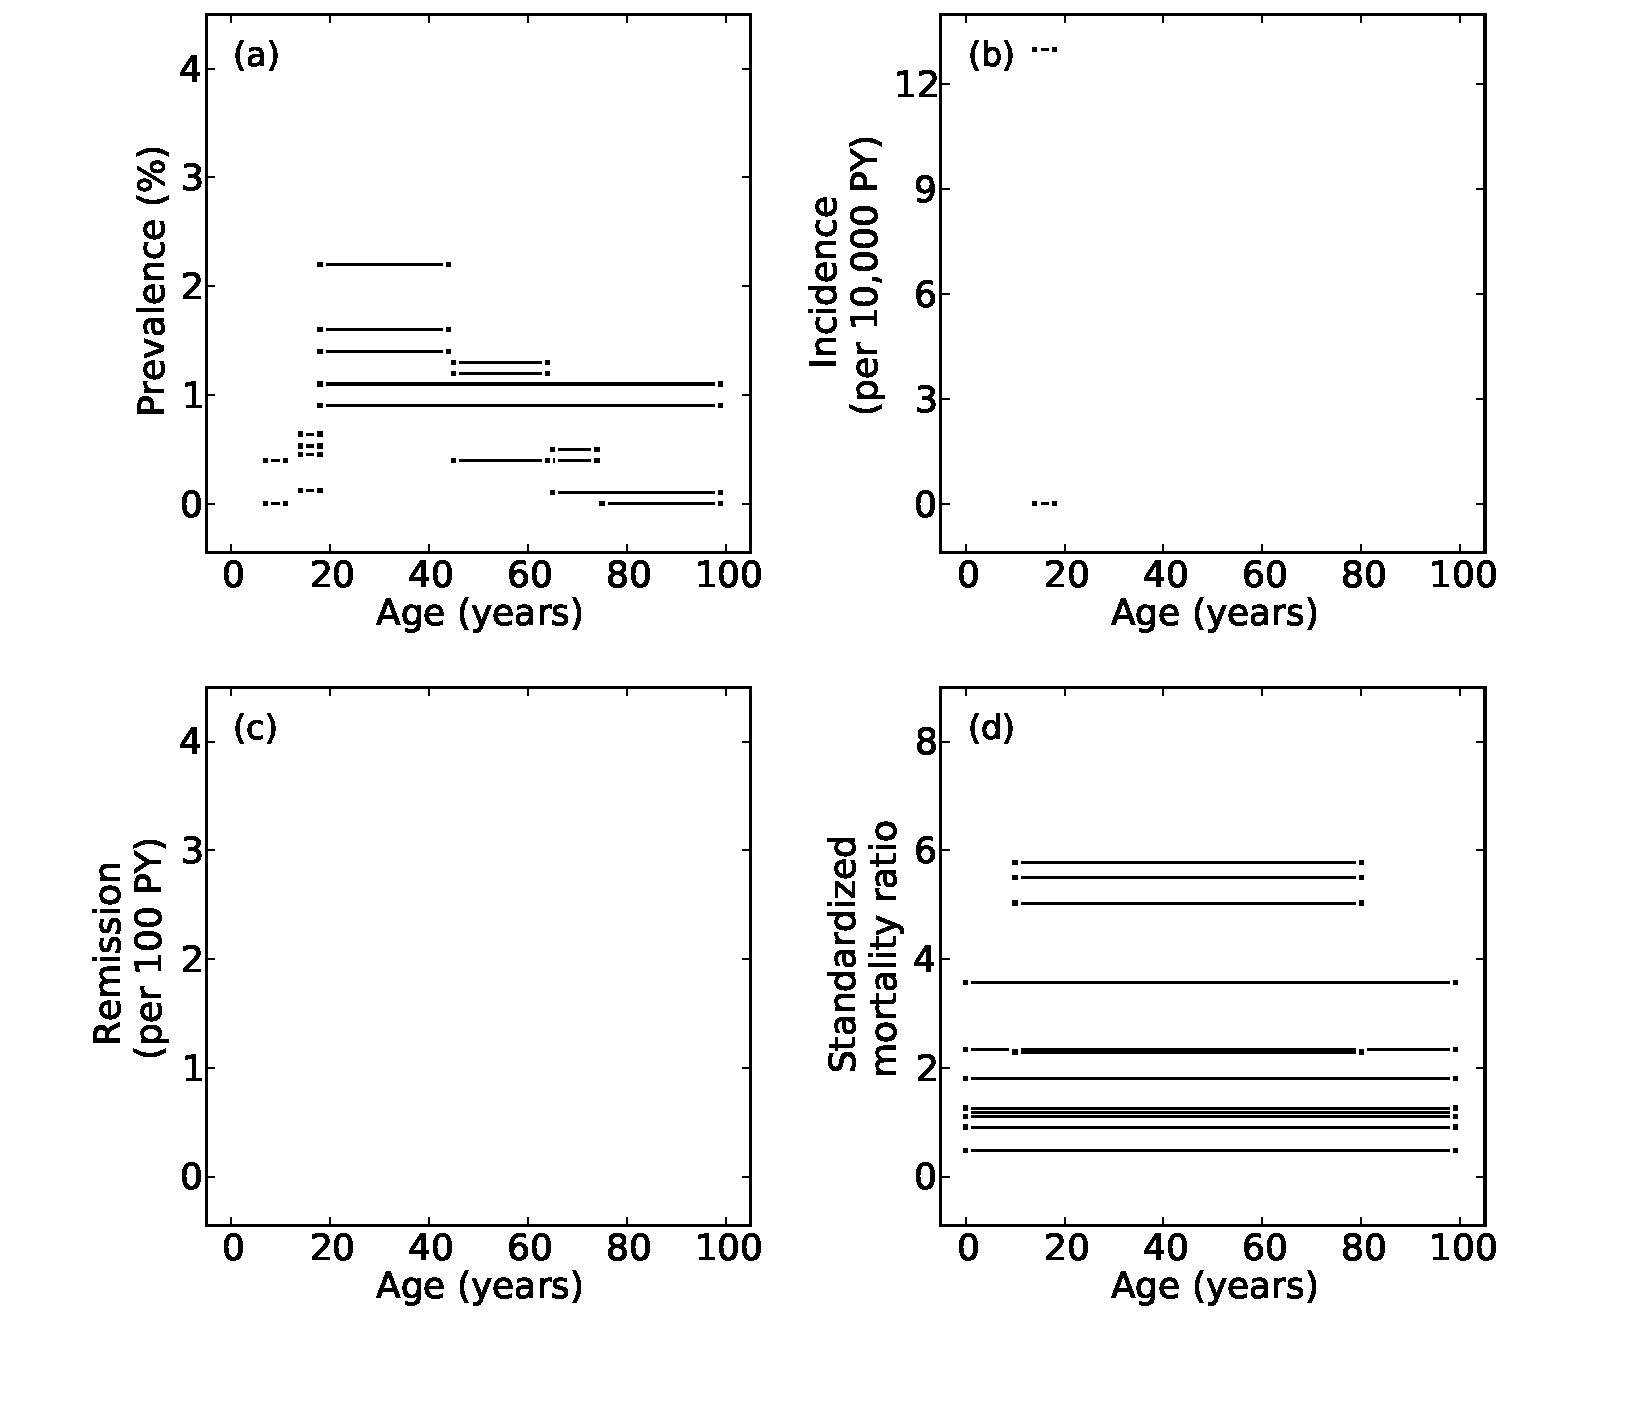
\includegraphics[width=\textwidth]{bipolar-data.pdf}
            \caption{Data included for the modeling of bipolar disorder.  Thirty-two studies were identified for prevalence, covering 22 countries in 11 GBD world regions.}
            \label{fig:app-bipolar data}
        \end{center}
    \end{figure}

\section{Prevalence and Incidence age of onset}
While there is evidence to suggest that bipolar disorder commonly starts in the mid-teens or early twenties, there is still disagreement over a minimum age of onset. Even though symptoms can be tracked back to childhood, setting a threshold for diagnosis is difficult given that current diagnostic criteria are based on adult presentation of the disorder. Literature and expert advice suggest that although pre-pubertal bipolar disorder is rare, there is a possibility it may exist \cite{angst_historical_2000}. Therefore a prior limiting age of onset to ages 10-90 was used.

    \begin{figure}[h]
        \begin{center}
            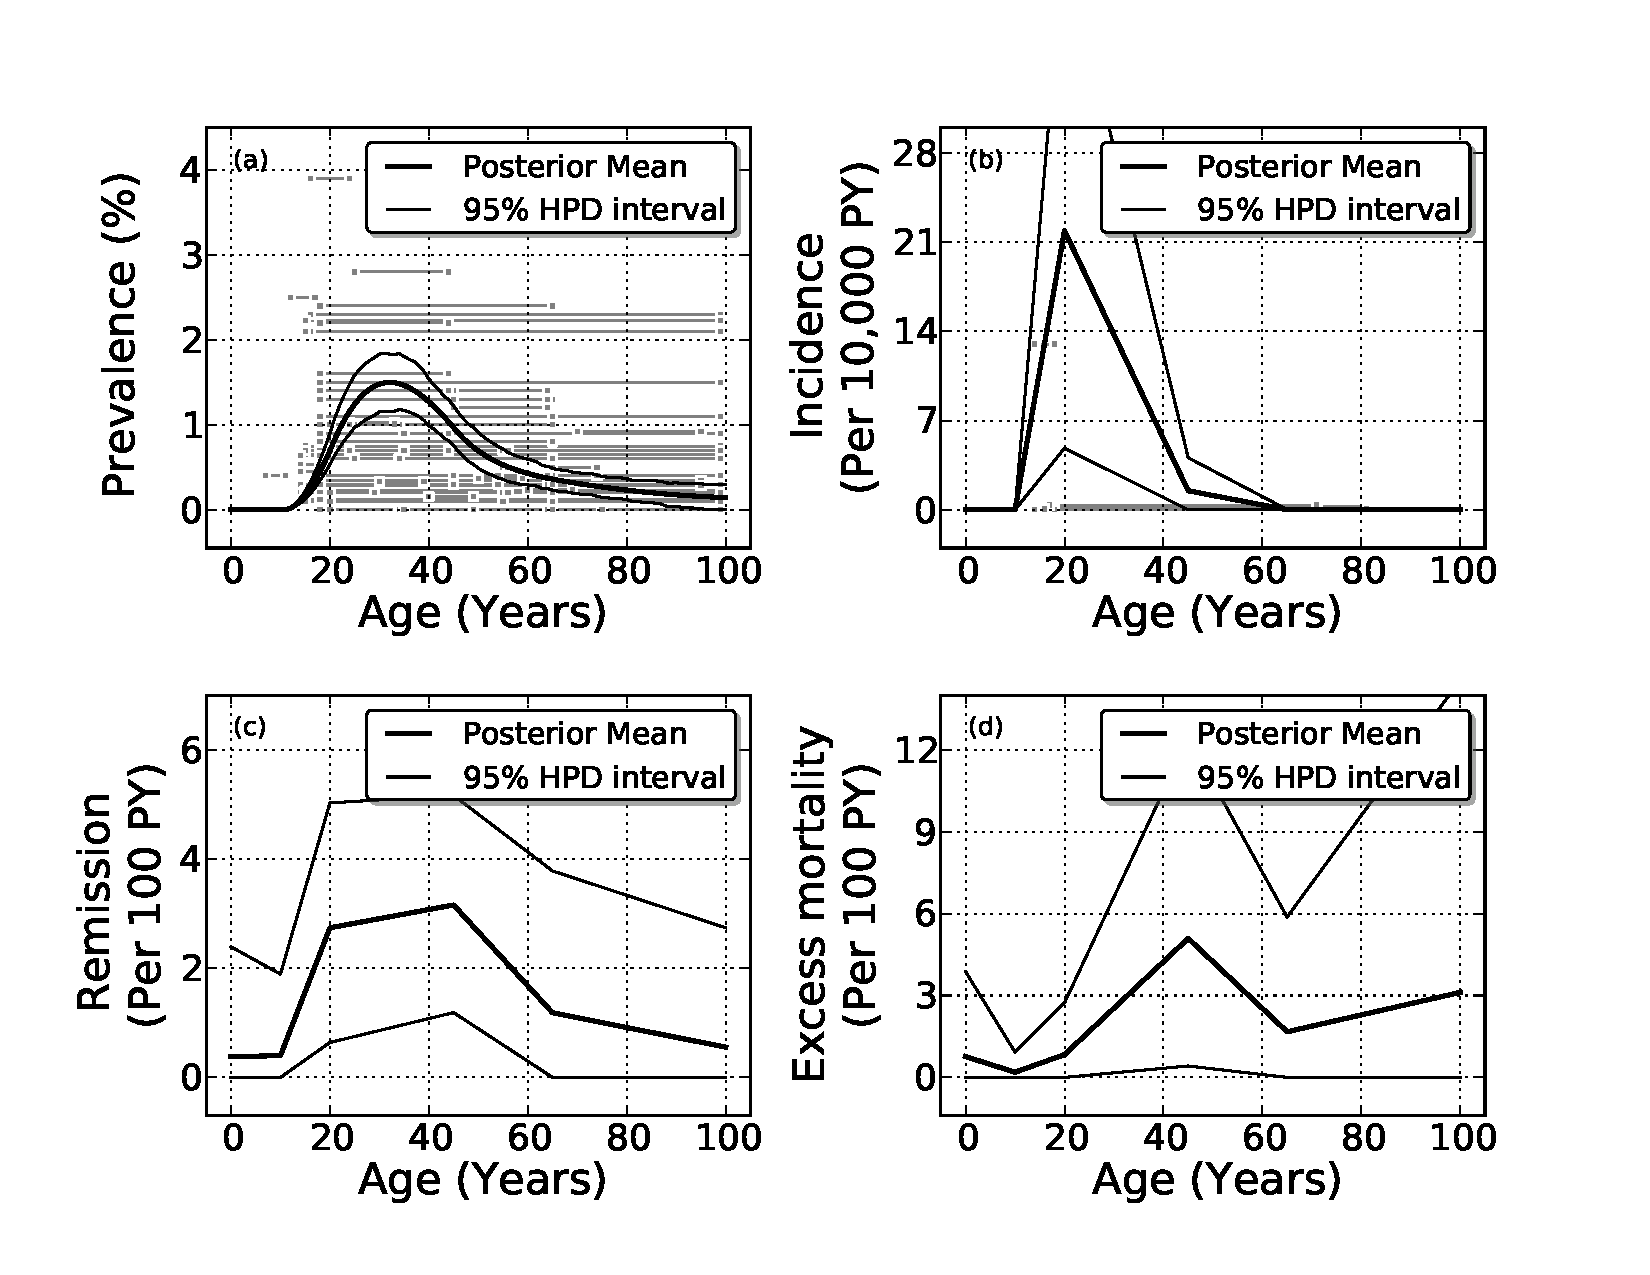
\includegraphics[width=\textwidth]{bipolar-zero_before_ten.pdf}
            \caption{Bipolar epidemiologic parameters for Western Europe males in 1990.  Priors set restrictions of the age of onset so that prevalence and incidence is 0 before age 10 and after age 65.}
            \label{fig:app-bipolar fit}
        \end{center}
    \end{figure}

While expert priors are useful in guiding the modeling process, they may have unintended effects as discussed in Chapter \ref{theory-expert_priors}.  Choosing to have no restrictions on the age of onset, the age-specific burden of disease differs greatly, as shown in figure \ref{fig:app-bipolar bounds}.

    \begin{figure}[h]
        \begin{center}
            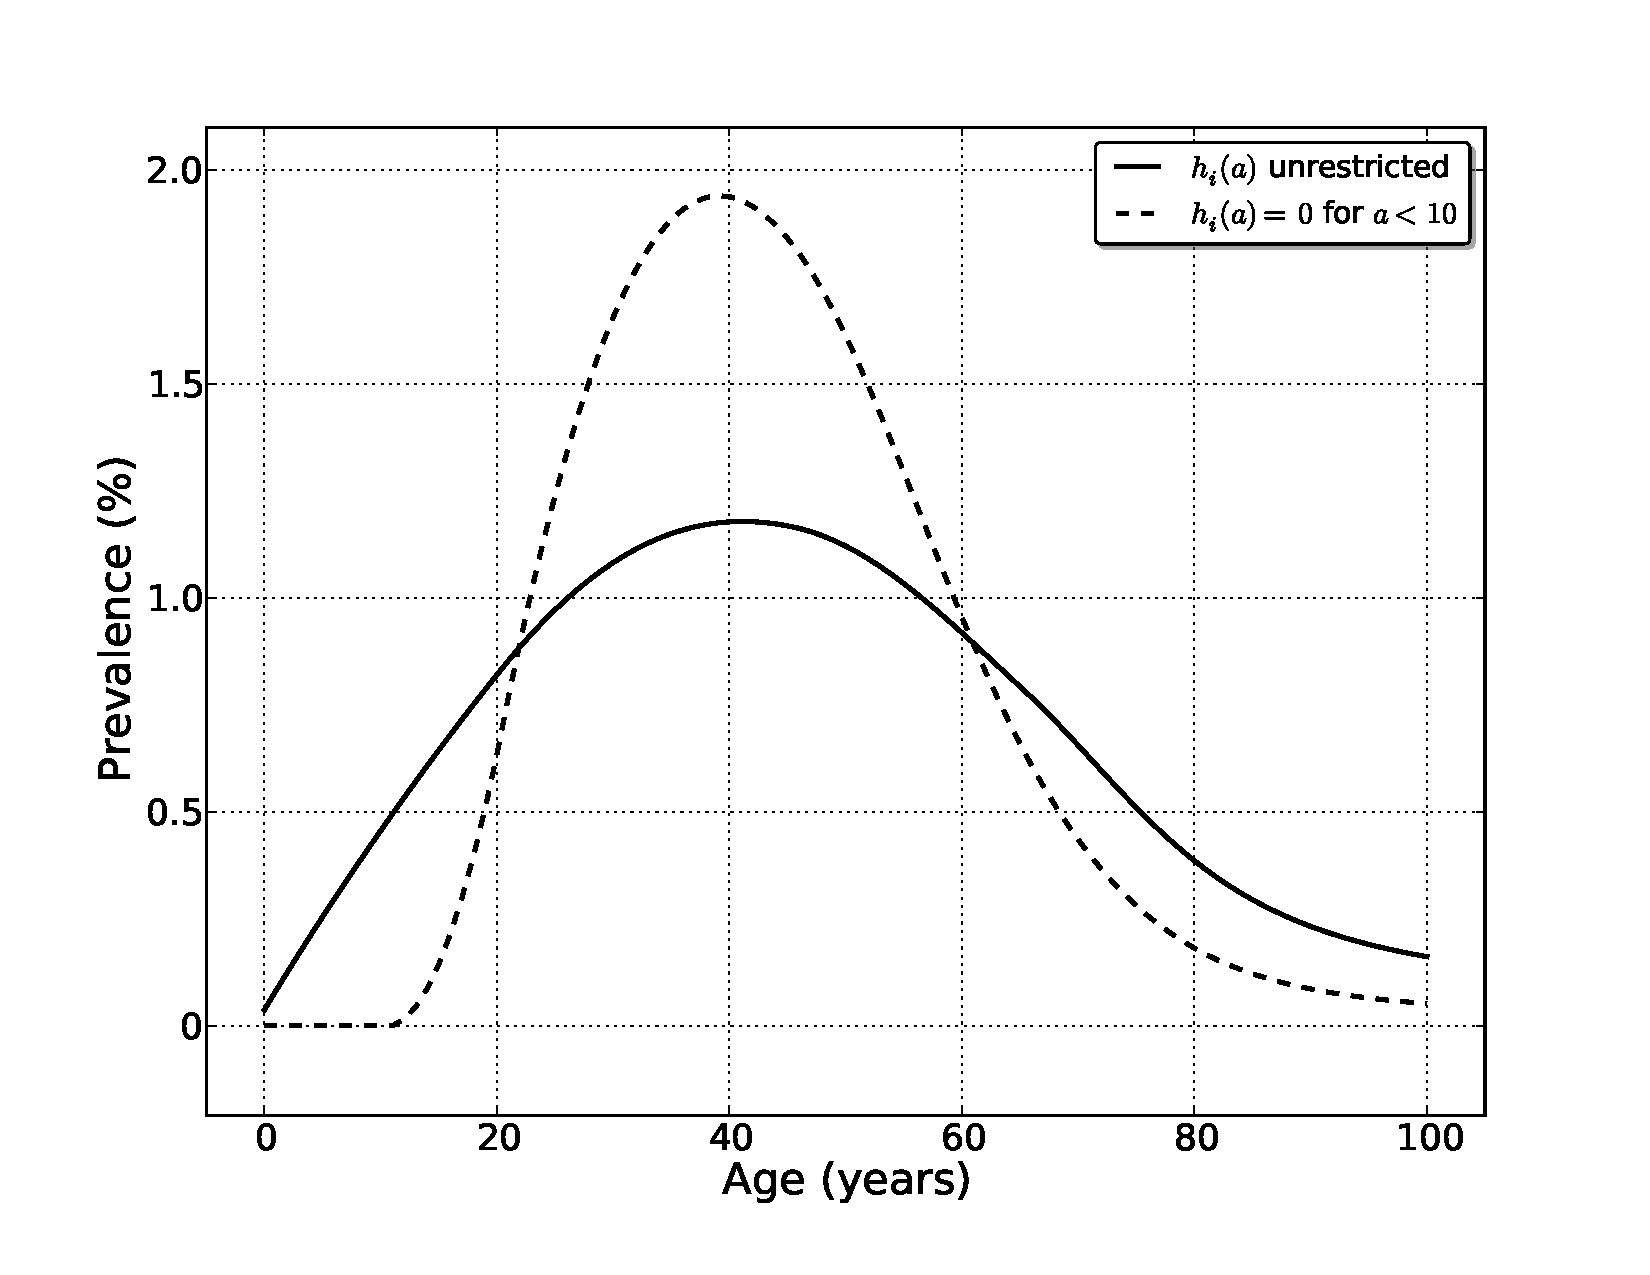
\includegraphics[width=\textwidth]{bipolar-bounds.pdf}
            \caption{Priors can have a large effect on the disease model.  Here, the prevalence of bipolar disorder in Western Europe males in 1990 differs greatly when there priors to limits age of onset.}
            \label{fig:app-bipolar bounds}
        \end{center}
    \end{figure}

Like the age of onset, little is known about the upper age limit of bipolar disorder.  Therefore a prior restricts the upper age limit to 65 years for incidence as it led to the most plausible fit to the data.  Using expert knowledge set plausible bounds on the level of disease is useful in modeling noisy data, but changes the upper age limit may produce unexpected changes as shown in figure \ref{fig:app-bipolar onset}.

    \begin{figure}[h]
        \begin{center}
            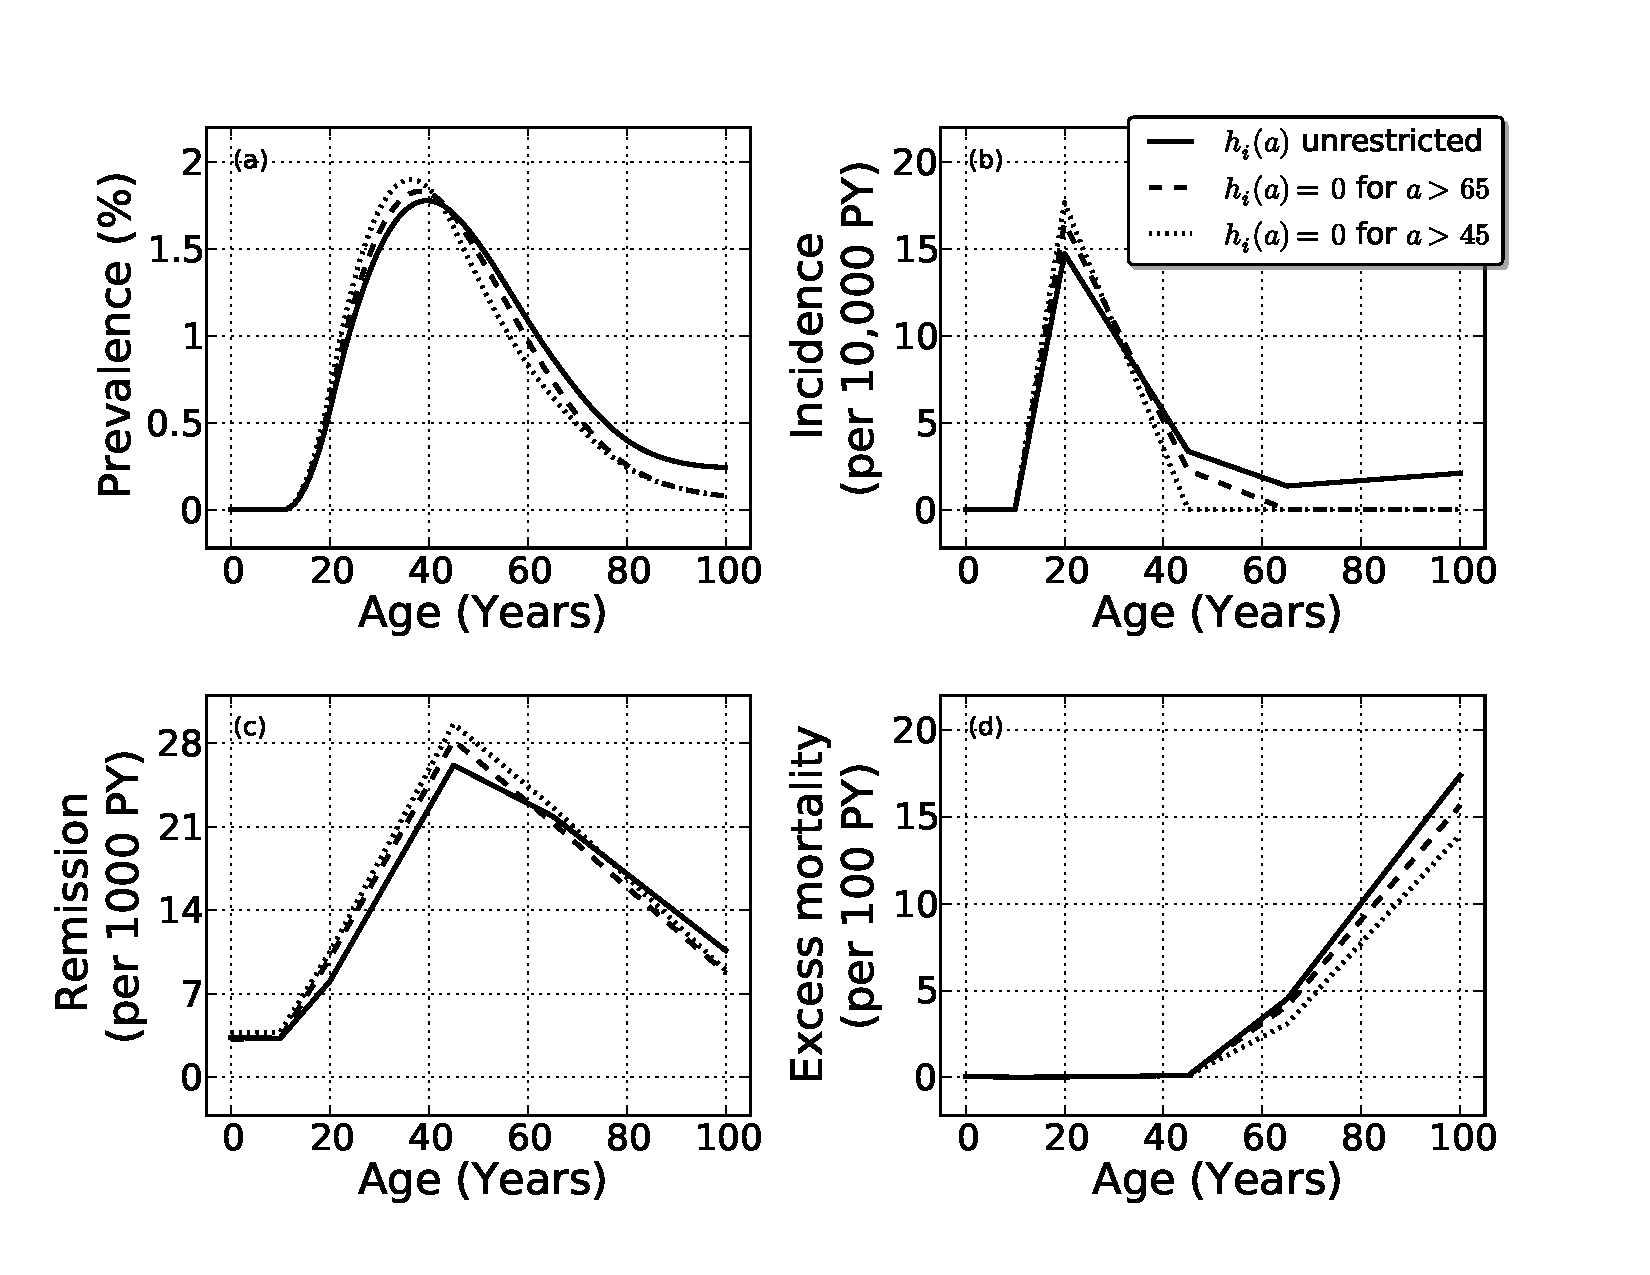
\includegraphics[width=\textwidth]{bipolar-45_65_100.pdf}
            \caption{Estimated prevalence, incidence, remission and excess mortality for Western Europe males with bipolar disorder in 1990.  Priors that restrict the upper age limit of incidence to 45, 65 and 100 propagate through the model to changes in remission and excess mortality.}
            \label{fig:app-bipolar onset}
        \end{center}
    \end{figure}

\section{Residual v Remission}
Although residual symptoms can be less severe than manic and depressive episodes, they still lead to some disability and therefore burden.  However since an average episode of bipolar disorder is believed to last for about 3 months or more, estimates of point prevalence assessing symptoms within the past month or less, will likely miss cases of bipolar disorder in a residual episode, thus underestimating prevalence \cite{angst_historical_2000}.

The terms `residual' and `remission' have very different implications for the GBD 2010 study.  A residual state involves mild symptoms with mild disability which still contribute to burden. Remission is equivalent to cure rather than a temporary reduction in symptom levels thus not contributing to burden. Since there is no consistent use of these terms in the bipolar literature, no remission data were included in the bipolar modeling. Instead, expert guidance set a level prior on the remission rate.  The compartmental model is sensitive to choice of prior. As shown in the figure \ref{fig:app-bipolar remission}, choice of prior leads to large changes in the estimated excess mortality.

    \begin{figure}[h]
        \begin{center}
            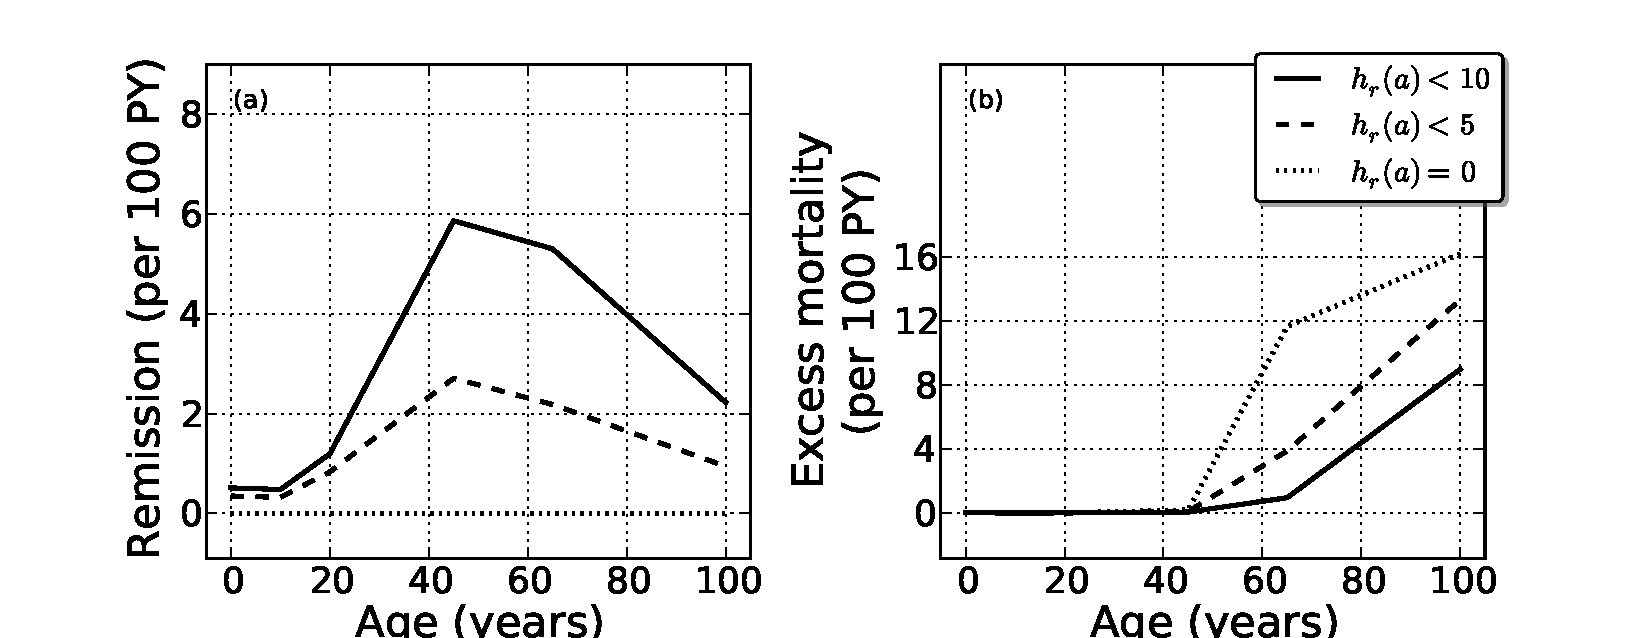
\includegraphics[width=\textwidth]{bipolar-0_5_10.pdf}
            \caption{With no data for bipolar disorder remission, a prior on the level of remission can have unexpected results, as shown above for Western Europe males in 1990.  Changing the remission prior levels for bipolar disorder also changes the excess mortality.}
            \label{fig:app-bipolar remission}
        \end{center}
    \end{figure}

